\documentclass[main]{subfiles}
\begin{document}
\begin{figure}
\caption{$V = \{2,3,5,8,11\}$}
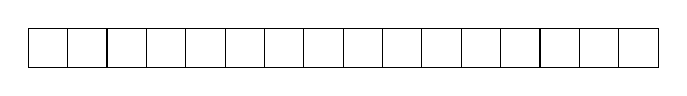
\begin{tikzpicture}[scale=0.5]
	\draw (0,0) grid (16,1);
	\putarray{0,0,1,1,0,1,0,0,1,0,0,1,0,0,0,0}
	%\node (a1) at (.5,.5) {0};
	%\node (a2) at (1.5,.5) {0};
	%\node (a3) at (2.5,.5) {1};
	%\node (a4) at (3.5,.5) {1};
	%\node (a5) at (4.5,.5) {0};
	%\node (a6) at (5.5,.5) {1};
	%\node (a7) at (6.5,.5) {0};
	%\node (a8) at (7.5,.5) {0};
	%\node (a9) at (8.5,.5) {1};
	%\node (a10) at (9.5,.5) {0};
	%\node (a11) at (10.5,.5) {0};
	%\node (a12) at (11.5,.5) {1};
	%\node (a13) at (12.5,.5) {0};
	%\node (a14) at (13.5,.5) {0};
	%\node (a15) at (14.5,.5) {0};
	%\node (a16) at (15.5,.5) {0};
\end{tikzpicture}
\end{figure}
\end{document}

